% !TeX spellcheck = en_US
\chapter{Unscharfe Daten und Fuzzy-Logik}
In dem normallen Alltag eines Menschen werden ständig Aussagen über Ereignisse getroffen. Diese Aussagen können möglichst exakt sein, oder auch nicht. In manchen Situationen werden solche genannt, die für den Menschen adäquat ein Ereignis beschreiben. Man würde zum Beispiel sagen, dass es gerade sehr stark regnet, oder es sehr heiß ist. Diese Information kann von dem menschlichen Gehirn angemessen vearbeitet werden. Maschinen, wie Komputern, sind jedoch nicht mit dieser Funktionalität ausgestattet. Die sogenannten unscharfe Daten müssen somit anders repräsentiert werden, damit auch Maschinen diese verarbeiten können. Auf dieser Weise können wir den Vorteil der Maschinen gegenüber Menschen ausnutzen - ihre große Kapazität und die Möglichkeit komplexere Strukturen und Systeme darzustellen. In diesem Kapitel wird eine Erweiterung der klassischen Logik vorgestellt, die es den Komputern ermöglicht, unscharfe Daten darzustellen und darauf Operationen durchzuführen. Diese Logik ist als Fuzzy-Logik bekannt.

\section{Fuzzy-Logik}

%Eine Menge beschreibt ein Zusammenhang von Elementen, oder Objekte. Jedes Element erf�llt eine bestimmte Eigenschaften. In der klassischen Mengenlehre geh�rt ein Element entweder vollst�ndig oder nicht.

In der Literatur bezeichnet man die präzise Darstellung von unscharfen Daten als Fuzzy-Logic. Fuzzy-Logic unterscheidet sich von der klassischen Mengenlehre darin, dass Elemente graduell einer Menge gehören und nicht nur bivalente Zugehörigkeit erweisen können.

Zum Verdeutlichen betrachten wir die Menge M der reellen Zahlen, die viel größer sind als 1. 

\begin{align}
\centering
	M = \{ x \ |\ x \in \Re,\ x >> 1\}
\end{align}

Wird diese Menge mit der klassischen Logik modelliert, ergibt sich die Problematik: Der Vergleich ``viel größer'' ist mathematisch nicht eindeutig definiert. Auf die Grafik unten kann man die Modellierung mit der klassischen Logik sehen.

%Hier Graphik f�r die Set mit klassiche Darstellung viel gr��er als 1

\begin{figure}[htbp]
	\centering
	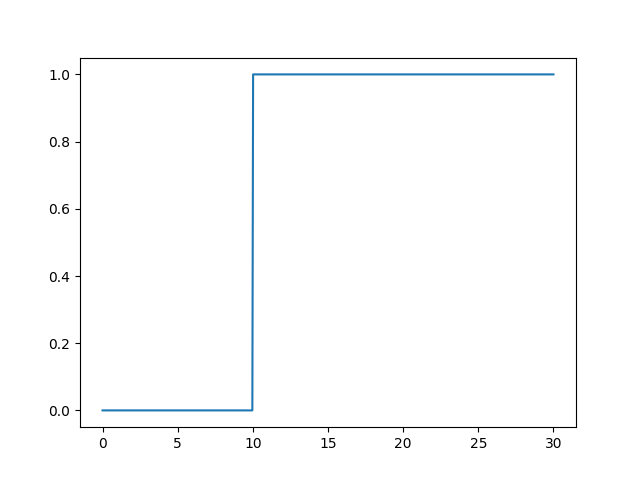
\includegraphics[scale=0.5]{images/classic_logic.png}
	\caption{``Viel größer als 1'' in der klassischen Logik}\label{class_dar}
\end{figure}

Aus der Graphik kann man feststellen, dass alle Werte kleiner als $10$ eine Zugehörigkeit von $0$ und solche größer oder gleich $10$ - eine Zugehörigkeit von $1$ besitzen. Diese Repräsentation entspricht jedoch die Realität nicht so ganz. Es ist eindeutig, dass ja $9.9$ als Wert schon größer als $1$ ist, aber der Graphik nach wird das nicht klar. Würde man diese Menge in der Fuzzy-Logik darstellen, ergibt sich folgendes Graph.

% Hier Graphik f�r die Fuzzy-Set "viel gr��er als 1"
\begin{figure}[htbp]
	\centering
	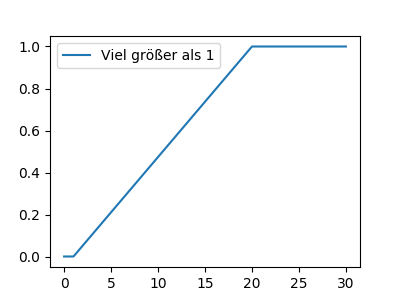
\includegraphics[scale=0.5]{images/fuzz_logic.png}
	\caption{``Viel größer als 1'' in der Fuzzy-Logik}\label{fuzzy_dar}
\end{figure}

Hier beschreibt die Graphik genauer, wie die Zahlen im Vergleich zu $1$ stehen. Die Zugehörigkeit nimmt Werte zwischen $0$ und $1$. Zum Beispiel der Wert $10$ hat die Zugehörigkeit von ca. $0.3$ und für Werte größer als $20$ liefert die Funktion $\mu (x)$ einen Wert von $1$ (volle Zugehörigkeit).


\subsection{Fuzzy-Sets}\label{fs_section}%Eventuell hier beschreiben
Fuzzy-Sets, oder Fuzzy-Mengen, beschreiben in der Fuzzy-Logik Eigenschaften von Elementen. Die Idee ist, dass Elemente zu einem rationallen Wert einer Menge gehören, beziehungsweise eine Eigenschaften besitzen. In der Literatur wird folgende Definition für Fuzzy-Mengen gegeben \cite{CIKruse:15}:

\begin{definition}
	Eine Fuzzy-Menge oder Fuzzy-Teilmenge $\mu$ der Grundmenge $X$ ist eine
	Abbildung $\mu : X \rightarrow [0, 1]$, die jedem Element $x \in X$ seinen Zugehorigkeitsgrad $\mu(x)$ zu
$\mu$ zuordnet. Die Menge aller Fuzzy-Mengen von $X$ bezeichnen wir mit $F(X)$. \cite{CIKruse:15}
\end{definition}

Normallen Mengen können als spezielle Fuzzy-Mengen aufgefasst werden. Also sind Fuzzy-Sets verallgemeinerte charakteristische Fuktionen \cite{CIKruse:15}.

In der Literatur tauchen unterschiedliche Arten von Fuzzy-Mengen. Die bekanntesten davon sind Dreiecksfunktion, Trapezfunktion und Gaußfunktion. Die Namensgebung kommt aus ihrer Form. Vier Beispielfunktionen sind unten gegeben.

\begin{figure}[htbp]
	\centering
	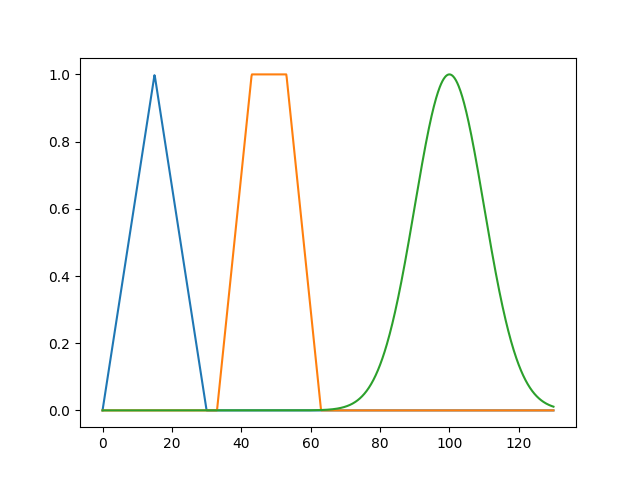
\includegraphics[scale=0.5]{images/mf_types.png}
	\caption{Arten von Fuzzy-Mengen}\label{mf_types}
\end{figure}

Die Form einer Fuzzy-Menge ist durch ihre Funktion bestimmt. Die Berechnung der Mengen wird folglich definiert.

\begin{equation}
	\mu_{tri}(x) = \begin{cases}
						\frac{x - a}{b - a} & \text{falls $a \leq x \leq b$}\\
						\frac{c - x}{c - b} & \text{falls $b \leq x \leq c$}\\
						0 & \text{sonst}
					\end{cases}
\end{equation}

Der Index der Funktion verdeutlicht, dass es sich um die Dreiecksfunktion handelt. Die Funktion hat drei Parametern, wo $a und c$ die Grenzenparametern sind und $b$ - der Gipfelpunkt. Außerdem muss $a < b < c$ gelten. Die Dreiecksfunktion ist ein besonderer Fall der Trapezfunktion, wo die Punkte, bzw. Parametern, der oberen Grudseite gleich sind. Deswegen ist die Gleichung \ref{trap_mf} für die Trapezfunktion sehr ähnlich \cite{CIKruse:15}.

\begin{equation}
\mu_{trap}(x) = \begin{cases}
\frac{x - a}{b - a} & \text{falls $a \leq x \leq b$}\\
1 & \text{falls $b \leq x \leq c$}\\
\frac{d - x}{d - c} & \text{falls $c \leq x \leq d$}\\
0 & \text{sonst}

\label{trap_mf}
\end{cases}
\end{equation}

Die Glockefunktion ist, wie ihrer Name andeutet, eine Funktion, die die Form einer Glocke hat. Die Darstellung dieser Funktion ähnelt sich sehr der Gaußsche Funktion. Die Berechnung wird untern gegeben. 

\begin{equation}
\mu_{bell}(x) = \frac{1}{1 + [(\frac{x - c}{a})^2]^b}
\label{bell_mf}
\end{equation}

Die letzte Funktion, die vorgestellt werden soll, ist die gaußsche Funktion. Die Formel wird öfters in der Statistik für Darstellung von Nominalverteilungen, aber auch in der Fuzzy-Logik. Die Gaußfunktion ist wie folgt definiert \cite{CIKruse:15}:

\begin{equation}
	\mu_{gauss}(x) = exp(\frac{-(x - m)^2}{s^2})
	\label{gauss_mf}
\end{equation}

Die Parametern $m und q$ sind entsprechend der Mittelwert (Mittelpunkt) und die Abweichung von der Mitte, oder als $\sigma$ (Sigma) in der Statistik bekannt.




%[Fuzzy-Logik und Fuzzy-Control, Jörg Kahlert; Hubert Frank,]
%
%
%   [Fuzzy-Logik und Fuzzy-Control, Jörg Kahlert; Hubert Frank, Computational Intelligence]

\section{Operationen auf Fuzzy-Sets}
In den vorherigen Kapiteln wurde auf die Wichtigkeit von Fuzzy-Logik, genau so wie Repräsentation von Fuzzy-Mengen eingegangen. Um nun unscharfe Informationen verarbeiten zu können, wie Schlüsse daraus zu ziehen oder mehrere Fuzzy-Mengen zu kombinieren, brauchen wir eine Reihe von Operatoren. Da es um Mengen geht, eignen sich die Durchschnitt-, Vereinigung- und Komplementbildung aus der klassischen Logik gut. Im folgenden Kapitel werden die einzelnen Operationen beschrieben [Computational Intelligence].

\subsection{Durchscnitt}\label{AND}

In der klassische Logik ist der Durchschnitt durch einen Logischen-UND eingesetzt. In der klassischen Mengenlehre ist die Menge aller Elementen, die zu einer Menge $M_1$ und einer Menge $M_2$ gehören, als Schnittmenge definiert. Gegeben seien die Mengen:

\begin{align}
M_1 = \{ x \ | \ x \in\Re, \ 1 \ \leq \ x \ \leq \ 3 \} 
\end{align}
\begin{align}
 M_2 = \{ x \ | \ x \in\Re, \ 2 \ \leq \ x \ \leq \ 4 \} 
\end{align}

Der Durchschnitt der beiden Mengen ergibt sich:

\begin{align}
M_1 \cap M_2 = \{ x \ | \ x \in \Re, \ 2 \ \leq \ x \ \leq \ 3 \}
\end{align} 

Der UND-Operator lässt sich analog auf die Fuzzy-Mengen anwenden. Es wird die Fläche bestimmt, die für beide Mengen erfüllt ist. Aus methematischer Sicht sprechen wir von dem Minimum-Operator(MIN).

%\theoremstyle{definition}
\begin{definition}
	Seien $\mu_1$ und $\mu_2$ zwei Fuzzy-Mengen auf der Grundmenge $G$. Dann heißt:
		\begin{center}
			$\mu_1$ $\cap$ $\mu_2$ : $G$ $\rightarrow$ [0,1] $\text{mit}$ ($\mu_1$ $\cap$ $\mu_2$)($x$) $=$ MIN($\mu_1$($x$) , $\mu_2$($x$)) 
		\end{center}
	der \textbf{Durchschnitt} der Fuzzy-Mengen $\mu_1$ und $\mu_2$.
\end{definition} 

Zur Veranschaulichung wird unten die Grafik angegeben. Da sind zwei Fuzzy-Sets dargestellt. Die zwei Ausdrücke, die betrachtet werden, sind $mittlere$ und $hohe$ Temperatur. Der rote gestrichene Bereich stellt die Ergebnismenge dar.

\begin{figure}[htbp]
	\centering
	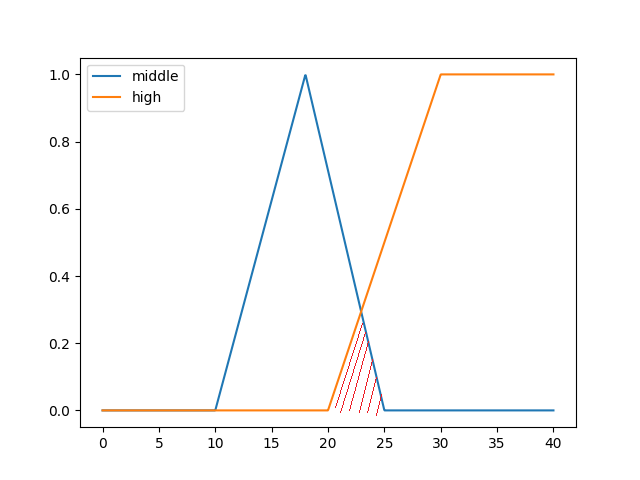
\includegraphics[scale=0.5]{images/und_high_middle_temp.png}
	\caption{Durchschnitt von zwei Fuzzy-Mengen (blauer gestrichener Bereich)}\label{high_low_temp_intersection}
\end{figure}

%hier Grafik f�r die Mittlere und Hohe Temperatur mengen.


\subsection{Vereinigung}

Nehmen wir ganz einfach die Definition der Vereinigung aus der klassischen Mengenlehre:
	\begin{center}
	$x$  $\in$ $M_1$ $\cup$ $M_2$ $\Leftrightarrow$ $x$ $\in$ $M_1$ $\vee$ $x$ $\in$ $M_2$
	\end{center}

Ziemlich eindeutig und klar. Die Vereinigungsmenge enthält alle diese Elemente aus dem Grundbereich, die entweder in der Menge $M_1$ oder $M_2$ enthalten sind. Im nächsten Schritt wird dieser Operator an die Fuzzy-Mengen angepasst.

In der Mathematik ist dieser Operator als ODER-Verknüpfung angegeben. Die Anwendung der ODER-Operator auf Fuzzy-Mengen wird wie folgt dann definiert:

%\theoremstyle{definition}

\begin{definition}
	Seien $\mu_1$ und $\mu_2$ zwei Fuzzy-Mengen auf der Grundmenge $G$. Dann heißt:
	\begin{center}
		$\mu_1$ $\cup$ $\mu_2$ : $G$ $\rightarrow$ [0,1] $\text{mit}$  ($\mu_1$ $\cap$ $\mu_2$)($x$) $=$ $MIN$($\mu_1$($x$)), $\mu_2$($x$)) 
	\end{center}
	die $\textbf{Vereinigung}$ der Fuzzy-Mengen $\mu_1$ und $\mu_2$.
\end{definition}

Betrachten wir den selben Beispiel aus vorherigen Unterkapitel. Seien also wieder die Fuzzy-Mengen für \textit{``mittlere''} und \textit{``hohe''} Temperatur. Wenn wir den ODER-Operator auf die beiden Mengen anwenden, ergibt sich eine Ergebnismenge, die sich auf beiden Mengenflächen aufstellt. Dies wurde graphisch zunächst aufgezeichnet.

\begin{figure}[htbp]
	\centering
	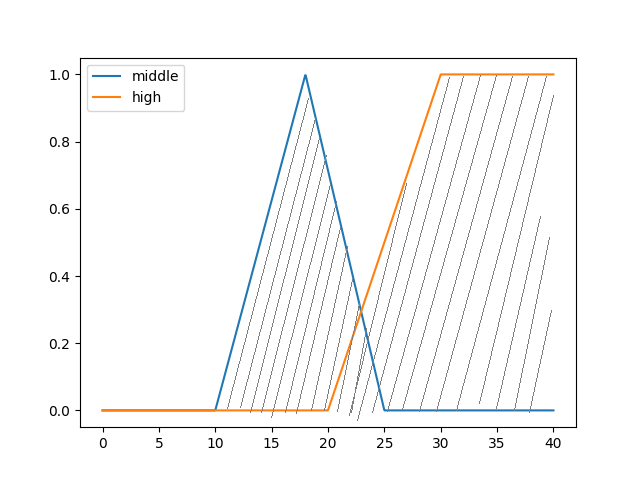
\includegraphics[scale=0.5]{images/oder_mid_high_temp.png}
	\caption{Union von Fuzzy-Mengen (gestrichener mit Rot Bereich)}
\end{figure}\label{high_low_temp_union}
% Hier Graphik f�r Oder verkn�pfung  

\subsection{Komplement}

Der dritte wichtige Operator ist das Komplement einer Menge. In der klassischen Mengenlehre ist dieser Operation ziemlich einfach anzuwenden. Der Operator beschreibt die Negation einer Aussage - zum Beispiel die Wahrscheinlichkeit eine 6 zu würfeln wäre $\frac{1}{6}$, die Gegenwahrscheinlichkeit, oder die Wahrscheinlichkeit etwas anderes als 6 zu würfeln wäre: (1 - $\frac{1}{6}$) = $\frac{5}{6}$. Das Komplement ist in der Fuzzy-Logik dann wie folgt definiert: 

\begin{definition}
	Sei $\mu$ eine Fuzzy-Menge auf der Grundmenge $G$. Dann heißt:
	\begin{center}
		$\mu^c$  : $G$ $\rightarrow$ [0,1] $\text{mit}$  ($\mu^c$)($x$) $=$ $1$ - $\mu$($x$)) 
	\end{center}
	die $\textbf{Vereinigung}$ der Fuzzy-Mengen $\mu_1$ und $\mu_2$.
\end{definition}

Zur Veranschaulichung die Menge \textit{hohe} Temperatur negiert. Die Negierung ist in der Graphik unten zu sehen.

%Hier Grafik f�r das Komplement-Beispiel

\begin{figure}[htbp]\label{not_high_temp}
	\centering
	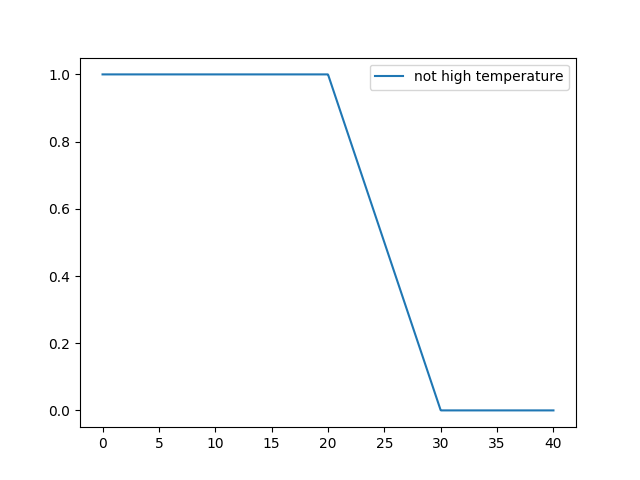
\includegraphics[scale=0.5]{images/not_high_temp.png}
	\caption{Komplement der Menge hohe Temperatur}
\end{figure}

\subsection{Zusammenfassung}

In diesem Kapitel habe ich die drei wichtigsten Operatoren auf Fuzzy-Mengen vorgestellt. Neben den Grundverknüpfungen gibt es eine weitere Sammlung von Verknüpfungsoperatoren.

\begin{enumerate}
	\item Algebraisches Produkt: ($\mu_1$$\mu_2$) = $\mu_1$($x$) $\cdot$ $\mu_2$($x$)
	\item direkte Summe: ($\mu_1$ $\bigoplus$ $\mu_2$) = $\mu_1$($x$) + $\mu_2$(x) - $\mu_1$($x$) $\cdot$ $\mu_2$($x$)
	\item abgeschnittene Differenz: ($\mu_1$ $\sqfrowneq$ $\mu_2$) = MAX(0, $\mu_1$(x) + $\mu_2$(x) - 1)
	\item abgeschnittene Summe: ($\mu_1$ \^{+} $\mu_2$) = MIN(1, $\mu_1$(x) + $\mu_2$(x))
	\item ($\mu_1$$\dotminus$ $\mu_2$) = MIN($\mu_1$(x), 1 - $\mu_2$(x))
	\item ...
\end{enumerate}

Dies ist eine Vorbereitung auf die folgenden Kapiteln. Wir analysieren mehrere Fuzzy-Mengen und ziehen daraus bestimmte Schlüsse. Ein Beispiel dafür wäre: Wenn eine Tomate rot ist, dann ist die reif. Folgende Logische Aussagen können sehr einfach mit Fuzzy-Logic modelliert werden. In der Literatur taucht die Name Fuzzy-Regeln. Diese können dann zusammengestellt werden, um Fuzzy-Regel-Systeme aufzubauen. Die nächste Kapitel stellt Fuzzy-Systeme vor. 

\section{Fuzzy-Systeme}

Ein Fuzzy-System, auch Fuzzy-Regler oder Fuzzy-Inferenz-System, ist ein bekannter Framework basierend auf Fuzzy-Mengen-Theorie, Fuzzy Wenn-Dann-Regeln und Fuzzy Reasoning. Konzeptionell besteht ein Fuzzy-System aus drei Grundteile - die Regelbasis, welche die Wenn-Dann-Regeln beinhaltet; die Datenbank(oder das Wörterbuch), die alle Zugehörigkeitsfunktionen definiert; und der Entscheidungmechanismus, wer die Inferenz durchführt und eine angemessene Schlussfolgerung erkundet.   

Folglich werden zwei Arten von Fuzzy-Systeme erläutert.

\subsection{Mamdani-Regler}

Der Mamdani-Regler wurde im Jahr 1975 von Mamdani auf der Basis einer Veröffentlichung von Zadeh aus der Anfang der siebziger Jahren entwickelt. 

Der Mamdani-Regler ist eine endliche Menge von Wenn-Dann-Regeln $R$ der Form:
\begin{equation}
	R: \text{If } x_1 \text{ is } A_1 \text{ and ... and } x_n \text{ is } A_n
	\text{ then } y^\prime \text{ is } B
\end{equation}

In der Regel sind $x_1$, ..., $x_n$ die Eingangsgrößen und $y^\prime$ die Ausgabe. $A_i$ und $B$ sind  linguistischen Werte. Jede Regel besteht aus zwei Teilen - Prämissen und Konklusionen. Jede Vorbedingung untersucht spezifische Eigenschaften. Es wird geprüft, ob der Eingangwert diese Eigenschaften erfüllt. Anhand diese Merkmale schließt sich eine Konklusion. 

Sei $W$ die Menge aller linguistischen Konklusionen $B_i$, so dass $B_1, \dots, B_m \in W$ gilt. Der Regler kann als eine n-Stellige Funktion mit $f: \mathbb{G^n} \mapsto W$ dargestellt werden. Die Funktion ordnet eine Eingabe zu einem linguistischen Term $B_i$.

\begin{equation}
	f(x_1, ..., x_n) \approx 
	\left\{
		\begin{array}{ll}
			B_1 & \mbox{ falls } x_1 \mbox{ is } A_1^{(1)} \mbox{ und ..., und } x_{n} \mbox{ is } A_n^{(1)}\\
			\vdots \\
			B_{m} & \mbox{ falls } x_1 \mbox{ is } A_1^{(m)} \mbox{ und ... und } x_{n} \mbox{ is } A_n^{(m)}
		\end{array}
	\right.
\end{equation}

In der Funktion gibt es genau so viele Ausgaben, wie es Regeln gibt - $m$.

Mit einem Mamdani-Regler können viele Probleme aus der reellen Welt definiert werden. Als kleines Beispiel eignet sich die Farben der Tomaten. Wir betrachten die Farbe als Eingabe. Die Ausgabe würde uns sagen, wie reif eine Tomate ist. Wir teilen unsere Eingangsgrößen in drei Farben: rot, gelb und grün. Daraus lassen sich entsprechend 3 Fuzzy-Mengen definieren. Als Ausgabe wird die Reife einer Tomate bestimmt. Das Ergebnis kann in drei Mengen anfallen: reif, halbreif oder unreif. Auf dieser Weise haben wir ein Mamdani-Fuzzy-Model, das aus 3 Fuzzy-Sets und aus 3 Regeln besteht. Die Regelbasis sieht wie folgt aus:

\begin{itemize}
	\item $R_1$: if x is rot, then y is reif.
	\item $R_2$: if x is gelb, then y is halbreif.
	\item $R_3$: if x is grün, then y is unreif.
\end{itemize}

Eine Tabelle für die Fuzzy-Relationen ist unten gegeben

\begin{table}\label{tomato:1}
	\centering
	\begin{tabular}{c|c c c}
		
		x \diagdown \ y & \ unreif & \ halbreif & \ reif \\ [0.5ex]
		\hline
		grün & 1 & 0 & 0 \\ 
		gelb & 0 & 1 & 0\\
		rot  & 0 & 0 & 1\\
		
	\end{tabular}
\caption{Beispiel für Tomaten}

\end{table}

Wie man sieht die Tabelle ist ziemlich einfach zu lesen, wenn die Tomate grün ist, wird immer angenommen dass sie unreif ist. Man könnte entsprechend die Fuzzy-Mengen aus der Konklusion verfeinern. Das würde bedeuten, dass die Mengen sich überlappen. Unsere Tabelle könnte dann wie folgt aussehen:

\begin{table}
	\centering
	\begin{tabular}{c|c c c}
		
		x \diagdown \ y & \ unreif & \ halbreif & \ reif \\ [0.5ex]
		\hline
		grün & 1 & 0.5 & 0 \\ 
		gelb & 0.3 & 1 & 0.3\\
		rot  & 0 & 0.5 & 1\\
		
	\end{tabular}
	\caption{Beispiel für Tomaten}
	\label{table:1}
\end{table}

Abhängig davon wie man die Ausgangsmengen definiert, wie weit die Mengen überlappen, ergibt sich eine unterschiedliche Interpretation der Werte. Je mehr Fuzzy-Sets für eine Größe(Maß) definiert sind, desto besser könnte ihr Zustand repräsentiert werden. Mit der Anzahl der Fuzzy-Sets steigt die Komplexität eines Systems proportional.

Den oberen kleinen Beispiel zeigt wie einfach Mamdani-Modelle zu modellieren sind. Mamdani-Reglern finden in der Praxis öfters Einsetzung.

\subsection{Takagi-Sugeno-Kang-Modell} \label{TSK}

Das Takagi-Sugeno-Kang-Modell ist dem Mamdani-Modell sehr ähnlich. TSK-Regler verwenden Regeln der Form:

\begin{align}
	R: \text{ If } x_1 \text{ is } \mu_R^{(1)} \text{ and \ldots and } x_n \text{ is } \mu_R^{(n)} \text{ then } y = f_R(x_1,\ldots,x_n).
\end{align}}

In den Prämissen ist kein Unterschied zu erkennen. Die Besonderheit des TSK-Modells liegt in der Konklusion. Da steht eine linear Funktion, anstatt eine Fuzzy-Menge. In der Konklusion kann im Allgemeinfall jede beliebige Funktion $f$ in der Eingabe von $x$ berechnet werden. Normalerweise ist $f$ eine linear Funktion, die wie folgt aussieht:
\begin{align}
	f(x_1, \ldots, x_n) = p_0 + p_1\cdot x_1 + \ldots + p_n\cdot x_n,
\end{align}
$p_0, \ldots, p_n$ sind die Parametern der Konklusionsfunktion. Für geiegnete ausgewählte Parameterwerte modelliert das TSK-Modell eine mathematische Funktion, dies kann z.B. die Quadratfunktion sein. Für den Fall, dass die Parametern $p_1, \ldots w_n$ den Wert 0 haben, erhält man einen Mamdani-Modell mit scharfer Ausgabe. Solche Modelle heißen in der Literatur auch \textbf{zero-order Sugeno-Fuzzy-Modelle} \cite{SCTemassi:01, NFMBothe:98, NFSC:97}.
Als Beispiel kann folgende Regelbasis betrachtet werden:
\begin{align}
R_1: \text{ If } x \text{ is ``sehr klein'' then } y = 0\\
R_2: \text{ If } x \text{ is ``klein'' then } y = 1\\
R_3: \text{ If } x \text{ is ``groß'' then } y = 2\\
R_4: \text{ If } x \text{ is ``sehr groß'' then } y = 3.
\end{align}
Die Fuzzy-Sets sind ``sehr klein'', ``klein'', ``groß'' und ``sehr groß'' und die Ergebnisswerte entsprechend \textit{0, 1, 2 und 3}.

\subsection{Fuzzifizierung und Defuzzifizierung}\label{FDF} 

Der Vorgang eines Modells zerlegt sich in zwei Teilen - Fuzzifizierung und Defuzzifizierung. Der erste Begriff beschreibt den Prozess für die Evaluierung der Eingangswerte in Fuzzyinferenzsysteme. Es gibt mehrere Evaluierungsmethoden, beziehungsweise Fuzzifizierungsmechanismen, wie zum Beispiel die Gaußsche Funktion (\ref{fs_section}). Der zweite Begriff bezeichnet die Vorgehensweise bei der Berechnung der Ausgabe, oder Inferenz, eines Fuzzy-Systems. Die Reihenfolge der beiden Prozesse ist somit bestimmt. Da im vorrigen Kapitel schon Beispiele für Fuzzifizierungsverfahren vorgestellt werden, steige ich demnächst in den unterschiedlichen Arten von Defuzzifizierung.

Bei der Regelaktivierung unterscheidet man zwei Fällen. Wenn die Eingabe einer volle Zugehörigkeit ergibt, dann liefert das Modell ganz normal den Wert der entsprechenden Konklusionsfunktion. Bei partielle Aktivierung mehreren Regeln ergibt sich das Inferenzergebnis aus einem spezifischen Verfahren. Dafür werden bestimmte Inferenzmethoden angewendet, zum Beispiel das Center of Gravity, oder Center of Area. Einige dieser Methoden werden inden folgenden Unterkapiteln vorgestellt. In allen Verfahren handelt es sich, um Mamdani-Reglern, wo die Konklusion einer Regel aus einer Fuzzy-Mengen besteht. Die letzte vorgestellte Methode ist spezifisch für Takagi-Sugeno-Kang-Modelle anzuwenden.

\subsubsection{Height Method}
Bei dieser Methode, auch als \textit{maximum membership principle} bekannt, wird der Regelaktievierung mit den größten Wert ausgewählt. Die Vorgehensweise könnte in Systeme verwendet werden, wo der größte Zutreffer nur wichtig ist. Als Beispiel könnte ein System mit entsprechenden Gegenmaßnahmen genannt werden, wo der größte Risiko Vorgang haben soll \cite{SCTemassi:01}.

\subsubsection{Center of Gravity}

Center of Gravity, auch als Center of Area bekannt, ist die prominenteste Methode von allen, wo sich das Ergebniss als schärfer Wert ergibt. Das Endergebniss berechnet sich aus folgender Formel:
\begin{align}
	y^* = \frac{\int y \cdot \mu_R(y)dy}{\int \mu_R(y)dy}
\end{align}

Der Wert \textit{y} hier ist das Ergebnis der aktivierte Regel \textit{R} und \textit{$y^*$} ist das Endergebniss. \cite{SCTemassi:01}

\subsubsection{Weighted Average Method}

Die gewichtete Durchschnittsmethode, oder Weighted Average Method, ist nur für Ausgangszugehörigkeitsfunktionen, die aus mehreren symmetrischen Zugehörigkeitsfunktionen $\mu_i$ besteht. Die Formel lautet:
\begin{align}
y^* = \frac{\sum_{i} \=y \cdot \mu_i(\=y)}{\sum \mu_i(\=y)}
\end{align}

Das Modus jeder Zugehörigkeitsfunktion $\mu_i$ wird duch den Wert von $\=y$ beschrieben. \cite{SCTemassi:01}

\subsubsection{Takagi-Sugeno-Kang-Defuzzifizierungsmethode}
Die Defuzzifizierungsmethode von TSK-Modelle berechnet eine Interpolation zwischen den Ausgangswerte. Die Formel nimmt den Ausgabewert jeder Regel und multipliziert den mit dem Gewicht, der Regelaktievierung, der entsprechenden Regel und gewichtet durch die Wahrheitsrate jeder Regel. Die Formel ist gegeben:
\begin{align}\label{TSK_defuzz}
y = \frac{\sum_{i} \mu_i \cdot f_i(x_1, ..., x_n)}{\sum \mu_i},
\end{align} wo $\mu_i$ die Wahrheitsrate, bzw. Aktievierungswert, einer Regel $i$ ist und $f_i$ liefert den Ergebniswert für die Regel bei Eingabe $x_1, ..., x_n$.

Zum Schluss wird eine Abbildung gegeben, die den gesammten Prozess, Fuzzifizierung und Defuzzifizierung, darstellt. Die Abbildung beschreibt, wie das Endergebnis berechnet wird.

\begin{figure}[htbp]
	\centering
	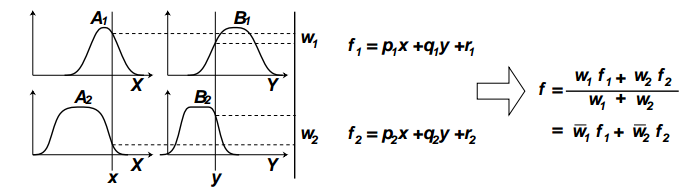
\includegraphics[scale=0.5]{images/TSK_Modell.png}
	\caption{Inferenzschritt eines TSK-Modells \cite{Jang:93}}\label{TSK_Modell}
\end{figure}

In der Figur wird ein Model mit zwei Eingangsgrößen und zwei Fuzzy-Mengen pro Eingabe dargestellt. Die Regelbasis besteht aus zwei Regeln und sind in der Reihe zu lesen. Die Fuzzy-Mengen werden durch die Glockefunktion berechnet. Die Variablen $w_1$ und $w_2$ liefern die Regelaktievierungen für die Regeln mit entsprechenden Indexen. Das Endergebnis $f$ ergibt sich aus der oben definierte Funktion \ref{TSK_defuzz}, wobei $w_1$ und $w_2$ der Variablen $\mu_1$ $\mu_2$ entsprechen.

%Unsicher ob ich darauf eingehen soll

%Die Gliederung h�ngt nat�rlich vom Thema und von der L�sungsstrategie ab. Als n�tzliche
%Anhaltspunkte k�nnen die Entwicklungsstufen oder - schritte z.B. der Softwareentwicklung betrachtet werden. N�tzliche Gesichtspunkte erh�lt und erkennt man, wenn man sich
%\begin{itemize}
%  \item in die Rolle des Lesers oder
%  \item in die Rolle des Entwicklers, der die Arbeit z.B. fortsetzen, erg�nzen oder pflegen soll,
%\end{itemize}
%versetzt. In der Regel wird vorausgesetzt, dass die Leser einen fachlichen Hintergrund haben - z.B. Informatik studiert haben. D.h. nur in besonderen, abgesprochenen F�llen schreibt man in popul�rer Sprache, so dass auch Nicht-Fachleute die Ausarbeitung prinzipiell lesen und verstehen k�nnen.
%
%Die �u�ere Gestaltung der Ausarbeitung hinsichtlich Abschnittformate, Abbildungen, mathematische Formeln usw. wird in \hyperref[Stile]{Kapitel~\ref*{Stile}} kurz dargestellt.